\chapter{Related Works}

Your related works, and your purpose and contribution which must be different as below.

\section{Same Topics}
Cite every latest journal with same topic
\subsection{Topic 1}
cite for first topic

\subsection{Topic 2}
if you have two topics you can include here to


\section{Same Method}
write and cite latest journal with same method

\subsection{Method 1}
cite and paraphrase method 1

\subsection{Method 2}
cite and paraphrase method 2 if you have more method please add new subsection.




 \section{Andri Fajar Sunandhar/1164065}
\subsection{binary classification dilengkapi ilustrasi gambar}
\begin{enumerate}
\item Binary classification yaitu berupa kelas positif dan kelas negatif. Klasifikasi biner adalah dikotomisasi yang diterapkan untuk tujuan praktis, dan dalam banyak masalah klasifikasi biner praktis, kedua kelompok tidak simetris - daripada akurasi keseluruhan, proporsi relatif dari berbagai jenis kesalahan yang menarik. Misalnya, dalam pengujian medis, false positive (mendeteksi penyakit ketika tidak ada) dianggap berbeda dari false negative (tidak mendeteksi penyakit ketika hadir).
\begin{figure}[ht]
\centering
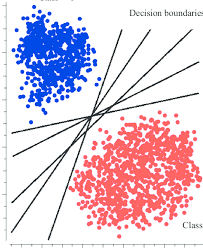
\includegraphics[scale=0.5]{figures/AFS/andri1.png}
\caption{Binary Classification}
\label{contoh}
\end{figure}
\end{enumerate}

\subsection{supervised learning dan unsupervised learning dan clustering dengan ilustrasi gambar}
\begin{enumerate}
\item Supervised learning adalah tugas pembelajaran mesin untuk mempelajari suatu fungsi yang memetakan input ke output berdasarkan contoh pasangan input-output. Ini menyimpulkan fungsi dari data pelatihan berlabel yang terdiri dari serangkaian contoh pelatihan. Dalam pembelajaran yang diawasi, setiap contoh adalah pasangan yang terdiri dari objek input (biasanya vektor) dan nilai output yang diinginkan (juga disebut sinyal pengawas). Algoritma pembelajaran yang diawasi menganalisis data pelatihan dan menghasilkan fungsi yang disimpulkan, yang dapat digunakan untuk memetakan contoh-contoh baru. Skenario optimal akan memungkinkan algoritma menentukan label kelas dengan benar untuk instance yang tidak terlihat. Ini membutuhkan algoritma pembelajaran untuk menggeneralisasi dari data pelatihan untuk situasi yang tidak terlihat dengan cara yang "masuk akal" (lihat bias induktif). Tugas paralel dalam psikologi manusia dan hewan sering disebut sebagai pembelajaran konsep. Contoh dibawah yaitu Supervised Learning dengan SVC.
\begin{figure}[ht]
\centering
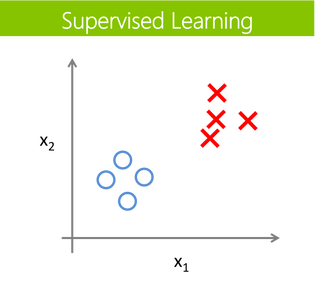
\includegraphics[scale=0.5]{figures/AFS/andri2.png}
\caption{Supervised Learning}
\label{contoh}
\end{figure}
\item Unsupervised learning adalah istilah yang digunakan untuk pembelajaran bahasa Ibrani, yang terkait dengan pembelajaran tanpa guru, juga dikenal sebagai organisasi mandiri dan metode pemodelan kepadatan probabilitas input. Analisis cluster sebagai cabang pembelajaran mesin yang mengelompokkan data yang belum diberi label, diklasifikasikan atau dikategorikan. Alih-alih menanggapi umpan balik, analisis klaster mengidentifikasi kesamaan dalam data dan bereaksi berdasarkan ada tidaknya kesamaan di setiap potongan data baru. BErikut merupakan contoh Unsupervised Learning dengan Gaussian mixture models.
\begin{figure}[ht]
\centering
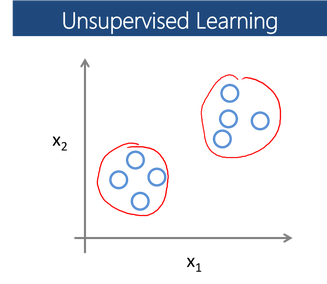
\includegraphics[scale=0.5]{figures/AFS/andri3.png}
\caption{Unsupervised Learning}
\label{contoh}
\end{figure}
\item Cluster analysis or clustering adalah tugas pengelompokan sekumpulan objek sedemikian rupa sehingga objek dalam kelompok yang sama (disebut klaster) lebih mirip (dalam beberapa hal) satu sama lain daripada pada kelompok lain (kluster). Ini adalah tugas utama penambangan data eksplorasi, dan teknik umum untuk analisis data statistik, yang digunakan di banyak bidang, termasuk pembelajaran mesin, pengenalan pola, analisis gambar, pengambilan informasi, bioinformatika, kompresi data, dan grafik komputer. Analisis Cluster sendiri bukan merupakan salah satu algoritma spesifik, tetapi tugas umum yang harus dipecahkan. Ini dapat dicapai dengan berbagai algoritma yang berbeda secara signifikan dalam pemahaman mereka tentang apa yang merupakan sebuah cluster dan bagaimana cara menemukannya secara efisien. Gagasan populer mengenai cluster termasuk kelompok dengan jarak kecil antara anggota cluster, area padat ruang data, interval atau distribusi statistik tertentu. Clustering karena itu dapat dirumuskan sebagai masalah optimasi multi-objektif. Algoritma pengelompokan dan pengaturan parameter yang sesuai (termasuk parameter seperti fungsi jarak yang akan digunakan, ambang kepadatan atau jumlah cluster yang diharapkan) tergantung pada set data individual dan penggunaan hasil yang dimaksudkan. Analisis kluster bukan merupakan tugas otomatis, tetapi proses berulang penemuan pengetahuan atau optimasi multi-objektif interaktif yang melibatkan percobaan dan kegagalan. Seringkali diperlukan untuk memodifikasi praproses data dan parameter model hingga hasilnya mencapai properti yang diinginkan.
\begin{figure}[ht]
\centering
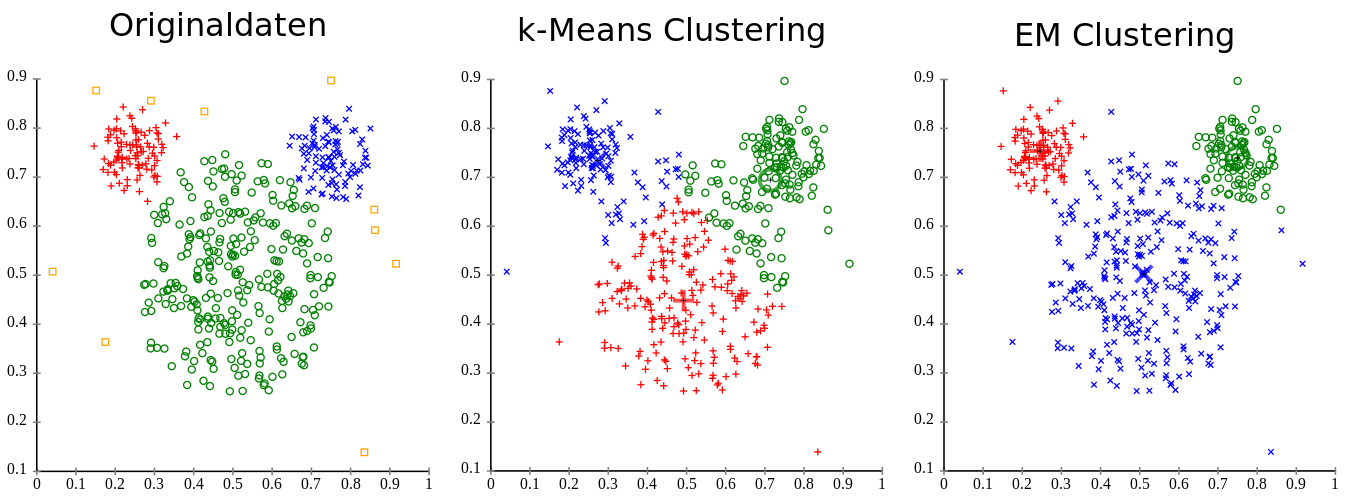
\includegraphics[scale=0.5]{figures/AFS/andri4.png}
\caption{Cluster}
\label{contoh}
\end{figure}
\end{enumerate}

\subsection{evaluasi dan akurasi dari buku dan disertai ilustrasi contoh
dengan gambar}
\begin{enumerate}
\item Evaluasi adalah tentang  bagaimana kita dapat mengevaluasi seberapa baik model bekerja dengan mengukur akurasinya. Dan akurasi akan didefinisikan sebagai persentase kasus yang diklasifikasikan dengan benar. Kita dapat menganalisis kesalahan yang dibuat oleh model, atau tingkat kebingungannya, menggunakan matriks kebingungan. Matriks kebingungan mengacu pada kebingungan dalam model, tetapi matriks kebingungan ini bisa menjadi sedikit sulit untuk dipahami ketika mereka menjadi sangat besar.
\begin{figure}[ht]
\centering
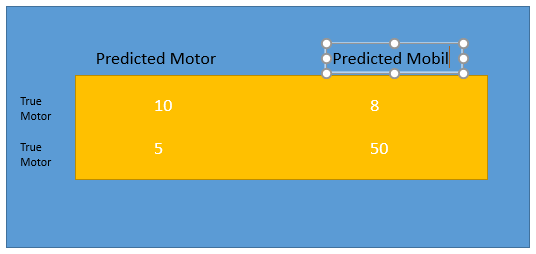
\includegraphics[scale=0.5]{figures/AFS/andri5.png}
\caption{ Evaluasi dan Akurasi}
\label{contoh}
\end{figure}
\end{enumerate}

\subsection{ bagaimana cara membuat dan membaca confusion matrix, buat confusion matrix }
\begin{enumerate}
\item Cara membuat dan membaca confusion matrix :
\begin{itemize}
\item 1)	Tentukan pokok permasalahan dan atributanya, misal gaji dan listik.
\item 2)	Buat pohon keputusan
\item 3)	Lalu data testingnya
\item 4)	Lalu mencari nilai a, b, c, dan d. Semisal a = 5, b = 1, c = 1, dan d = 3.
\item 5)	Selanjutnya mencari nilai recall, precision, accuracy, serta dan error rate.
\end{itemize}
\item Berikut adalah contoh dari confusion matrix :
\begin{itemize}
\item Recall =3/(1+3) = 0,75
\item Precision = 3/(1+3) = 0,75
\item Accuracy =(5+3)/(5+1+1+3) = 0,8
\item Error Rate =(1+1)/(5+1+1+3) = 0,2
\end{itemize}
\end{enumerate}

\subsection{bagaimana K-fold cross validation bekerja dengan gambar ilustrasi}
\begin{enumerate}
\item Cara kerja K-fold cross validation :
\begin{itemize}
\item 1)	Total instance dibagi menjadi N bagian.
\item 2)	Fold yang pertama adalah bagian pertama menjadi data uji (testing data) dan sisanya menjadi training data.
\item 3)	Lalu hitung akurasi berdasarkan porsi data tersebut dengan menggunakan persamaan.
\item 4)	Fold yang ke dua adalah bagian ke dua menjadi data uji (testing data) dan sisanya training data. 
\item 5)	Kemudian hitung akurasi berdasarkan porsi data tersebut.
\item 6)	Dan seterusnya hingga habis mencapai fold ke-K.
\item 7)	Terakhir hitung rata-rata akurasi K buah.
\end{itemize}
\begin{figure}[ht]
\centering
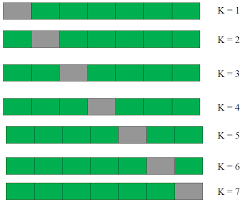
\includegraphics[scale=0.5]{figures/AFS/andri6.png}
\caption{K-fold cross validation }
\label{contoh}
\end{figure}
\end{enumerate}

\subsection{decision tree dengan gambar ilustrasi}
\begin{enumerate}
\item Decision Tree dalah metode pembelajaran yang diawasi non-parametrik yang digunakan untuk klasifikasi dan regresi. Tujuannya adalah untuk membuat model yang memprediksi nilai variabel target dengan mempelajari aturan keputusan sederhana yang disimpulkan dari fitur data.\\
Misalnya, dalam contoh di bawah ini, decision tree belajar dari data untuk memperkirakan kurva sinus dengan seperangkat aturan keputusan if-then-else. Semakin dalam pohon, semakin rumit aturan keputusan dan semakin bugar modelnya.
\begin{figure}[ht]
\centering
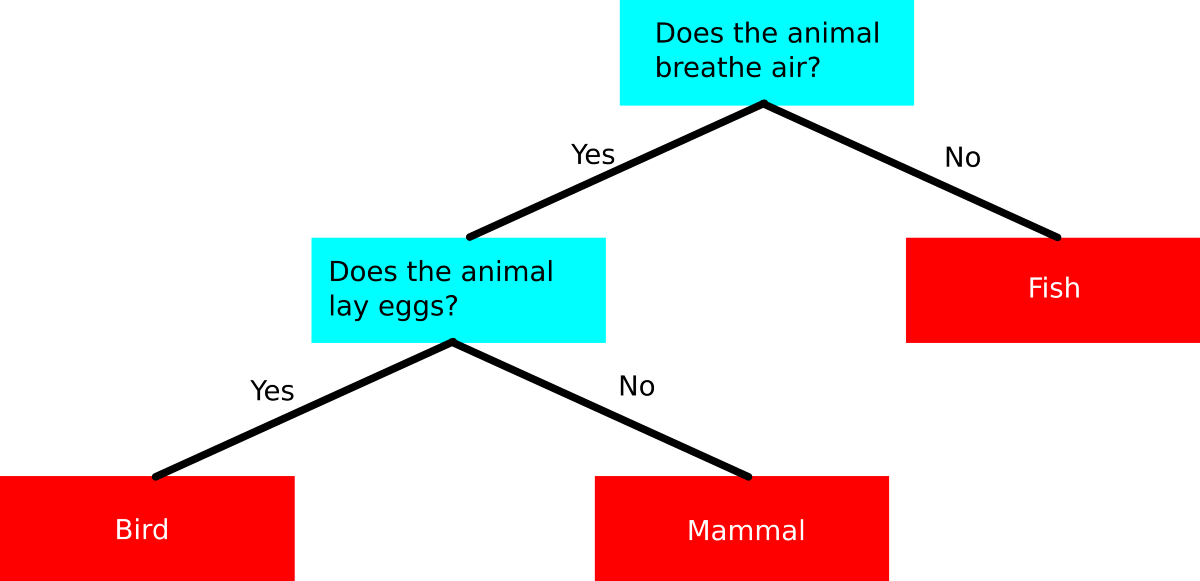
\includegraphics[scale=0.5]{figures/AFS/andri7.png}
\caption{Decision Tree}
\label{contoh}
\end{figure}
\end{enumerate}

\subsection{Information Gain dan entropi dengan gambar ilustrasi}
\begin{enumerate}
\item Information gain didasarkan pada penurunan entropi setelah dataset dibagi pada atribut. Membangun decision tree adalah semua tentang menemukan atribut yang mengembalikan perolehan informasi tertinggi (mis., Cabang yang paling homogen).
\begin{figure}[ht]
\centering

\includegraphics[scale=0.5]{figures/AFS/andri8.png}
\caption{Information gain}
\label{contoh}
\end{figure}
\item Entropi adalah ukuran keacakan dalam informasi yang sedang diproses. Semakin tinggi entropi, semakin sulit untuk menarik kesimpulan dari informasi itu. Membalik koin adalah contoh tindakan yang memberikan informasi yang acak. Untuk koin yang tidak memiliki afinitas untuk kepala atau ekor, hasil dari sejumlah lemparan sulit diprediksi. Mengapa? Karena tidak ada hubungan antara membalik dan hasilnya. Inilah inti dari entropi.
\end{enumerate}

\section{scikit-learn}
HARI KEDUA ANDRI FAJAR SUNANDHAR 1164065

\begin{enumerate}

\item
\begin{verbatim}
	# load dataset (student Portuguese scores)
	import pandas as apel
	jeruk = apel.read_csv('E:\KAMPUS\Semester 6\Kecerdasan Buatan\modul\Python-Artificial-Intelligence-Projects-for-			 	Beginners\Chapter01\dataset\student-mat.csv', sep=';')
	len(jeruk)
\end{verbatim}

\par
Untuk mengimport atau memanggil module pandas sebagai apel. Kemudian mendefinisikan variabel "jeruk" yang akan memanggil dataset yang didapatkan dari data student-mat.csv 
\begin{figure}[ht]
\centering
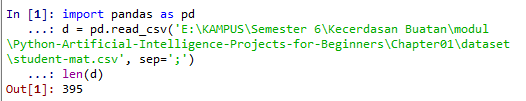
\includegraphics[scale=0.5]{figures/spyder/1.png}
\caption{Loading Dataset}
\label{Spyder}
\end{figure}
\item
\begin{verbatim}
	# generate binary label (pass/fail) based on G1+G2+G3 (test grades, each 0-20 pts); threshold for passing is sum>=30
	jeruk['pass'] = jeruk.apply(lambda row: 1 if (row['G1']+row['G2']+row['G3']) >= 35 else 0, axis=1)
	jeruk = jeruk.drop(['G1', 'G2', 'G3'], axis=1)
	jeruk.head()
\end{verbatim}

\par
mendeklarasikan label pass/fail nya data berdasarkan G1+G2+G3. 
kemudian pada variabel jeruk dideklarasikan  jika baris dengan G1+G2+G3 ditambahkan, dan hasilnya sama dengan 35 maka axisnya 1. 
\begin{figure}[ht]
\centering
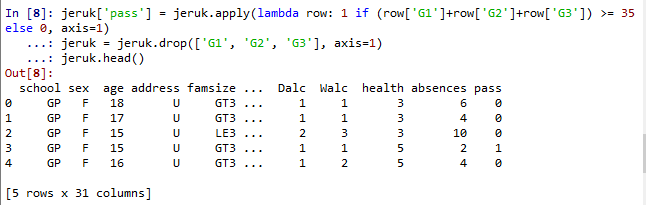
\includegraphics[scale=0.5]{figures/spyder/2.png}
\caption{Generate Binary Label}
\label{Spyder}
\end{figure}
\item
\begin{verbatim}
	# use one-hot encoding on categorical columns
	jeruk = apel.get_dummies(jeruk, columns=['sex', 'school', 'address', 'famsize', 'Pstatus', 'Mjob', 'Fjob', 
                               'reason', 'guardian', 'schoolsup', 'famsup', 'paid', 'activities',
                               'nursery', 'higher', 'internet', 'romantic'])
	jeruk.head()
\end{verbatim}
\par
One-hot encoding adalah proses di mana variabel kategorikal dikonversi menjadi bentuk yang dapat disediakan untuk algoritma .
\begin{figure}[ht]
\centering
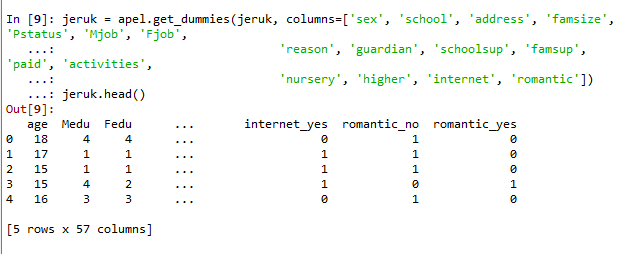
\includegraphics[scale=0.5]{figures/spyder/3.png}
\caption{One-hot Encoding}
\label{Spyder}
\end{figure}
\item
\begin{verbatim}
	# shuffle rows
	jeruk = jeruk.sample(frac=1)
	# split training and testing data
	jeruk_train = jeruk[:500]
	jeruk_test = jeruk[500:]

	jeruk_train_att = jeruk_train.drop(['pass'], axis=1)
	jeruk_train_pass = jeruk_train['pass']

	jeruk_test_att = jeruk_test.drop(['pass'], axis=1)
	jeruk_test_pass = jeruk_test['pass']

	jeruk_att = jeruk.drop(['pass'], axis=1)
	jeruk_pass = jeruk['pass']

	# number of passing students in whole dataset:
	import numpy as np
	print("Passing: %d out of %d (%.2f%%)" % (np.sum(jeruk_pass), len(jeruk_pass), 100*float(np.sum(jeruk_pass)) / 	len(jeruk_pass)))
\end{verbatim}

\par
 Pada bagian tersebut, terdapat train dan test yaing digunakan untuk untuk membagi train, test dan kemudian membagi lagi train ke validasi dan test.\\
Kemudia akan mengimport module numpy sebagai np yang akan digunakan untuk mengembalikan nilai passing dari pelajar dari keseluruhan dataset dengan cara print.
\begin{figure}[ht]
\centering
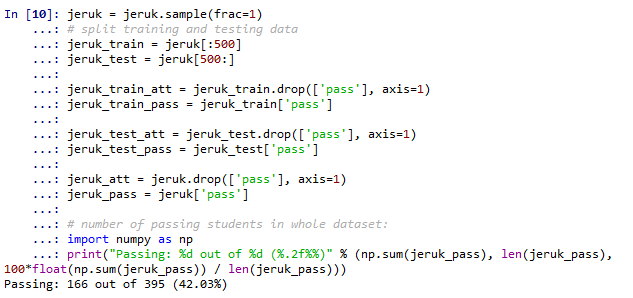
\includegraphics[scale=0.5]{figures/spyder/4.png}
\caption{Shuffle Rows}
\label{Spyder}
\end{figure}
\item 
\begin{verbatim}
	# fit a decision tree
	from sklearn import tree
	semangka = tree.DecisionTreeClassifier(criterion="entropy", max_depth=5)
	semangka = semangka.fit(jeruk_train_att, jeruk_train_pass)
\end{verbatim}

\par
Dari librari scikitlearn import modul tree. Kemudian definisikan variabel semangka dengan menggunakan DecisionTreeClassifier. Kemudian pada variabel semangka terdapat Criterion , setelah itu agar DecisionTreeClassifier dapat dijalankan gunakan perintah fit. hasilnya seperti dibawah
\begin{figure}[ht]
\centering
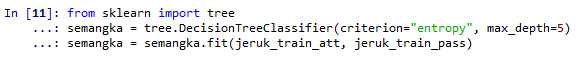
\includegraphics[scale=0.5]{figures/spyder/5.png}
\caption{Fit Decision Tree}
\label{Spyder}
\end{figure}
\item
\begin{verbatim}
	# visualize tree
	import graphviz
	dot_data = tree.export_graphviz(semangka, out_file=None, label="all", impurity=False, proportion=True,
                                feature_names=list(jeruk_train_att), class_names=["fail", "pass"], 
                                filled=True, rounded=True)
	graph = graphviz.Source(dot_data)
	graph
\end{verbatim}

\par
Mengimport Graphviz Sehingga akan muncul gambardiagram  grafik bercabang.
\begin{figure}[ht]
\centering
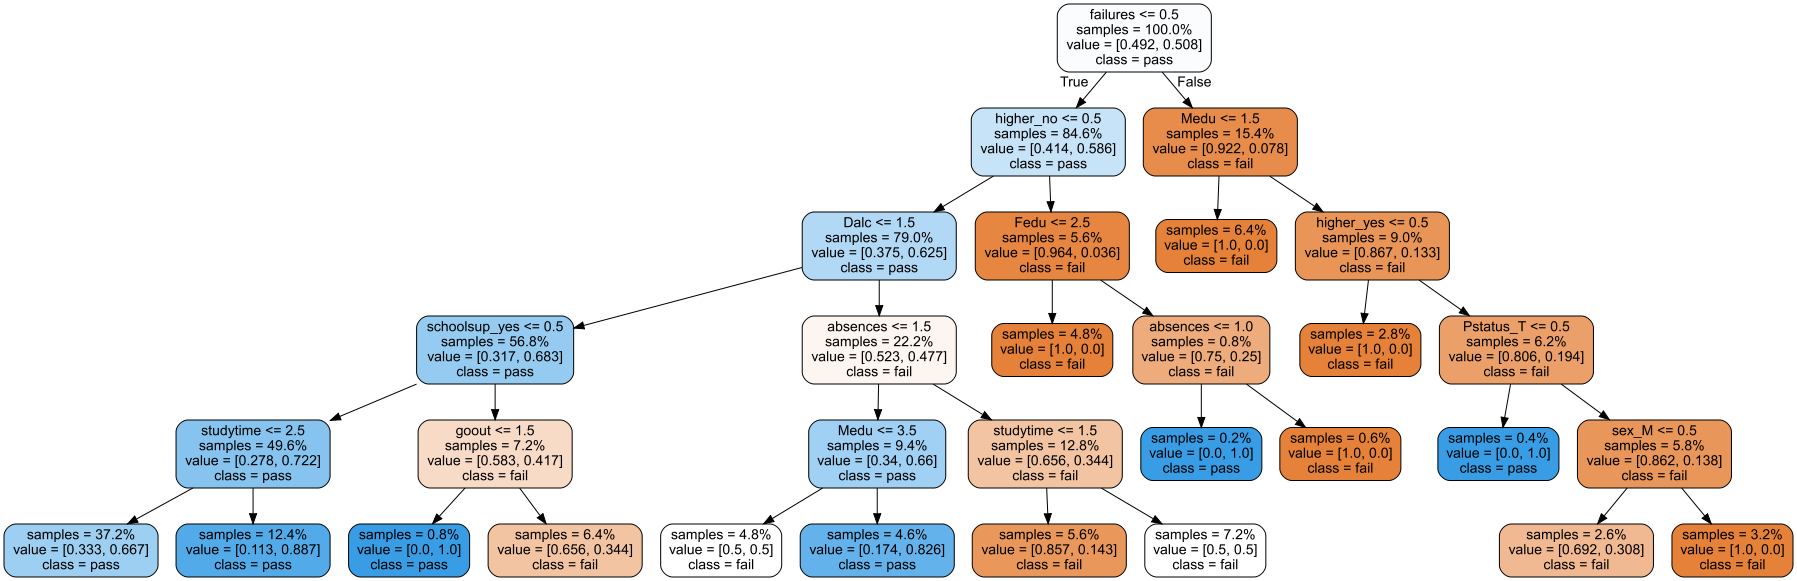
\includegraphics[scale=0.5]{figures/spyder/6.png}
\caption{Fit Decision Tree}
\label{Spyder}
\end{figure}
\item
\begin{verbatim}
	# save tree
	tree.export_graphviz(semangka, out_file="student-performance.dot", label="all", impurity=False, proportion=True,
                     feature_names=list(jeruk_train_att), class_names=["fail", "pass"], 
                     filled=True, rounded=True)
\end{verbatim}

\par
tree.exportgraphviz merupakan fungsi yang menghasilkan representasi Graphviz dari decision tree.
\begin{figure}[ht]
\centering
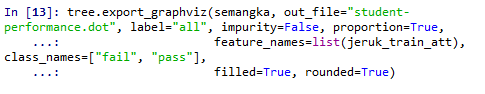
\includegraphics[scale=0.5]{figures/spyder/7.png}
\caption{Fit Decision Tree}
\label{Spyder}
\end{figure}
\item
\begin{verbatim}
	semangka.score(jeruk_test_att, jeruk_test_pass)
\end{verbatim}

\par
Score juga disebut prediksi, Nilai atau skor yang dibuat dapat mewakili prediksi nilai masa depan, tetapi mereka juga mungkin mewakili kategori atau hasil yang mungkin. disini semangka akan memprediksi jeruk.
\begin{figure}[ht]
\centering
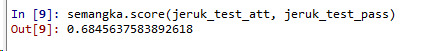
\includegraphics[scale=0.5]{figures/spyder/88.jpeg}
\caption{Score}
\label{Spyder}
\end{figure}
\item
\begin{verbatim}
	from sklearn.model_selection import cross_val_score
	scores = cross_val_score(semangka, jeruk_att, jeruk_pass, cv=5)
	# show average score and +/- two standard deviations away (covering 95% of scores)
	print("Accuracy: %0.2f (+/- %0.2f)" % (scores.mean(), scores.std() * 2))
\end{verbatim}

\par
 Dari sklearn.modelselection akan mengimport crossvalscore. Kemudian akan menampilkan score rata rata dan kurang lebih dua standar deviasi yang mencakup 95 persen score.
\begin{figure}[ht]
\centering
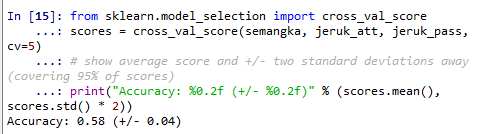
\includegraphics[scale=0.5]{figures/spyder/9.png}
\caption{Cross Val Score}
\label{Spyder}
\end{figure}
\item 
\begin{verbatim}
	for max_depth in range(1, 20):
   	 semangka = tree.DecisionTreeClassifier(criterion="entropy", max_depth=max_depth)
    	scores = cross_val_score(semangka, jeruk_att, jeruk_pass, cv=5)
    	print("Max depth: %d, Accuracy: %0.2f (+/- %0.2f)" % (max_depth, scores.mean(), scores.std() * 2))
\end{verbatim}

\par
Semangka akan mendefinisikan tree.DecissionTreeClassifier nya yang kemudian variabel semangka akan mengevaluasi score dengan validasi silang.
\begin{figure}[ht]
\centering
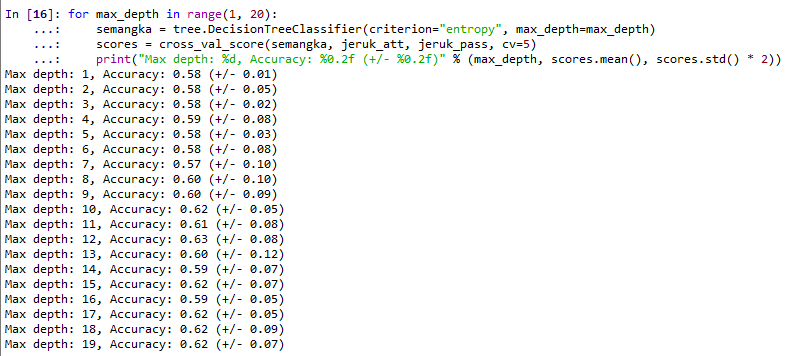
\includegraphics[scale=0.5]{figures/spyder/10.png}
\caption{Max Depth}
\label{Spyder}
\end{figure}
\item
\begin{verbatim}
	depth_acc = np.empty((19,3), float)
	i = 0
	for max_depth in range(1, 20):
    	semangka = tree.DecisionTreeClassifier(criterion="entropy", max_depth=max_depth)
    	scores = cross_val_score(semangka, jeruk_att, jeruk_pass, cv=5)
   	 depth_acc[i,0] = max_depth
   	 depth_acc[i,1] = scores.mean()
   	 depth_acc[i,2] = scores.std() * 2
   	 i += 1
    
	depth_acc

\end{verbatim}

\par
Dengan 19 sebagai bentuk array kosong, 3 sebagai output data-type dan float urutan kolom-utama (gaya Fortran) dalam memori. variabel semangka yang akan melakukan split score dan nangka akan mengvalidasi score secara silang. 
\begin{figure}[ht]
\centering
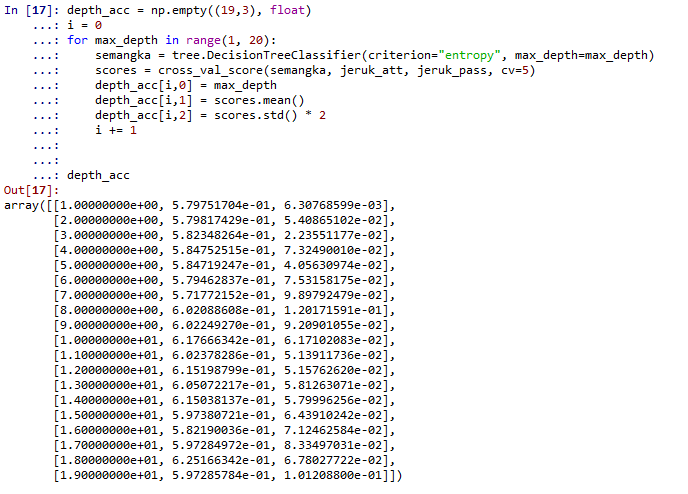
\includegraphics[scale=0.5]{figures/spyder/11.png}
\caption{Depth in Range}
\label{Spyder}
\end{figure}
\item 
\begin{verbatim}
	import matplotlib.pyplot as plt
	fig, ax = plt.subplots()
	ax.errorbar(depth_acc[:,0], depth_acc[:,1], yerr=depth_acc[:,2])
	plt.show()
\end{verbatim}

\par
Mengimpor librari dari matplotlib yaitu pylot sebagai plt\\
fig dan ax menggunakan subplots untuk membuat gambar .\\
ax.errorbar akan membuat error bar
\\
\\
\\
\begin{figure}[ht]
\centering
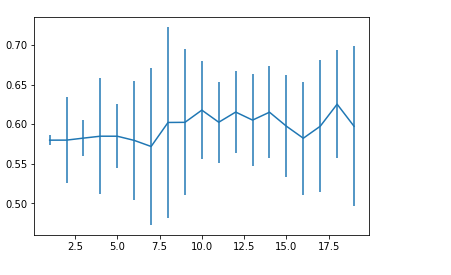
\includegraphics[scale=0.5]{figures/spyder/12.png}
\caption{Matplotlib}
\label{Spyder}
\end{figure}
\end{enumerate}

\section{Penanganan Error}
Hari Kedua Andri fajar Sunandhar 1164065
\subsection{Error Graphviz}
\begin{enumerate}
	\item
error yang didapatkan saat menjalankan Graphviz
\begin{figure}[ht]
\centering
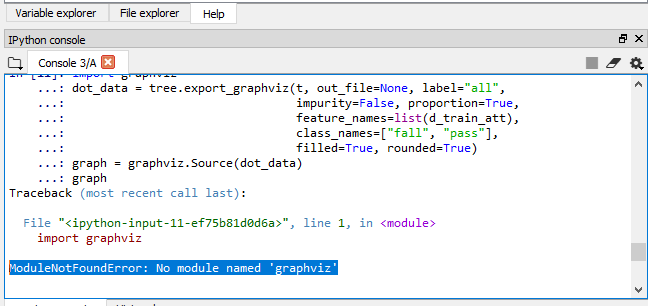
\includegraphics[scale=0.5]{figures/spyder/20.png}
\caption{Error Graphviz}
\label{Error}
\end{figure}
	\item
Kode erornya adalah ModuleNotFoundError. Eror ini terjadi karena module named Graphviz nya tidak ada.
	\item
Solusi yang bisa dilakukan untuk mengatasi eror tersebut adalah sebagai berikut : \\
\begin{itemize}
\item
buka CMD kemudian perintah pip install graphviz
\begin{figure}[ht]
\centering
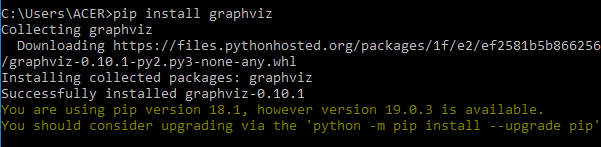
\includegraphics[scale=0.5]{figures/spyder/21.png}
\caption{install Graphviz}
\label{solusi}
\end{figure}
\item
masukan perintah conda install pip, untuk solving environment
\begin{figure}[ht]
\centering
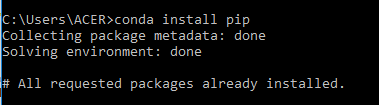
\includegraphics[scale=0.5]{figures/spyder/22.png}
\caption{Solving Environment}
\label{solusi}
\end{figure}
\item
selanjutnya masukan perintah conda install python-graphviz , untuk menambahkan package python-graphviz pada conda
\begin{figure}[ht]
\centering
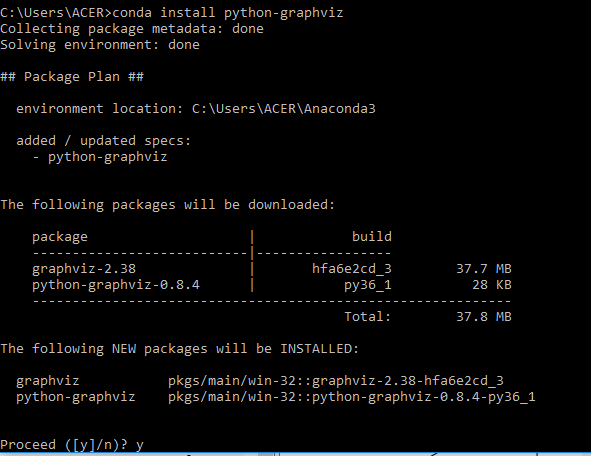
\includegraphics[scale=0.5]{figures/spyder/23.png}
\caption{Evaluasi Eror}
\label{Eror}
\end{figure}
\end{itemize}
\end{enumerate}

